\chapter{Greedy Algorithm}

\section{Maximal Matching}

\begin{algoprob}
	\problemtitle{Maximal-Matching}
	\probleminput{Graph $G=(V,E)$}
	\problemquestion{Find a maximal matching $M\subseteq E$ of $G$}
\end{algoprob}
Before diving into the algorithm to find a matching or maximal matching we first define what is a matching.
\begin{Definition}{Matching}{}
	For a graph $G=(V,E)$ a matching $M\subseteq E$ is a set of edges such that no two edges in $M$ are incident on same vertex.
\end{Definition}
\begin{Definition}{Maximal Matching}{}
	For a graph $G=(V,E)$ a matching $M\subseteq E$ is maximal if it cannot be extended and still by adding an edge.
\end{Definition}
There is also a maximum matching which can be easily understood from the name:
\begin{Definition}{Maximum Matching}{}
	For a graph $G=(V,E)$ a matching $M\subseteq E$ is maximum if it is maximal and has the maximum size among all the maximal matchings.
\end{Definition}

\begin{idea*}
	The idea is to create a maximal matching we will just go over each edge one by one and check if after adding them to the set $M$  the matching property still holds. 
\end{idea*}
\begin{algorithm}
	\SetKwComment{Comment}{// }{}
	\DontPrintSemicolon
	\KwIn{Graph $G=(V,E)$}
	\KwOut{Maximal Matching $M\subseteq E$ of $G$}
	\Begin{
	$M\longleftarrow \emptyset$\;
	Order the edges $E=\{e_1,\dots, e_k\}$ arbitrarily\;
	\For{$e\in E$}{\If{$M\cup \{u\}$ is matching}{$M\longleftarrow M\cup \{e\}$}}
	\Return{$M$}	
}
\caption{\prb{Maximal-Matching}}
\end{algorithm}

\begin{question}{}{}
		Do we always get the largest possible matching?
\end{question}
\solve{ Clearly algorithm output is not optimal always. We get a maximal matching sure. But we don't get a maximum matching always. For example the following graph
	\begin{center}
		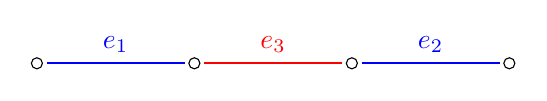
\begin{tikzpicture}
			\draw (-2,0) circle (2pt) node (A){};
			\draw (0,0) circle (2pt) node (B){};
			\draw (2,0) circle (2pt) node (C){};
			\draw (4,0) circle (2pt) node (D){};
			\draw[blue, thick] (A) -- node[midway, above]{$e_1$} (B);
			\draw[red, thick] (B) -- node[midway, above]{$e_3$}(C);
			\draw[blue, thick] (C) -- node[midway, above]{$e_2$} (D);
		\end{tikzpicture}
	\end{center}
	If we start from $e_1$ we get the matching $\{e_1.e_2\}$ which is maximum matching but if we start from $e_3$ then we get only the maximal matching $\{e_3\}$ which is not maximum.}

 Since the algorithm output may not be optimal always we can ask the following question
 \begin{question}{}{}
 	How large is the matching obtained compared to the maximum matching?
 \end{question}
This brings us to the following result:

\begin{Theorem}{}{}
	For any graph $G$ let the greedy algorithm obtains the matching $M$ and the maximum matching is $M^{\star}$. Then $$|M|\geq \frac12|M^\star|$$
\end{Theorem}
\begin{proof}
	content...
\end{proof}
\section{Huffman Encoding}
\begin{algoprob}
	\problemtitle{Huffman-Coding}
	\probleminput{$n$ symbols $A=(a-1,\dots, a_n)$ and their frequencies $P=(f_1,\dots, f_n)$ of using symbols}
	\problemquestion{Create a binary encoding such that: \begin{itemize}[itemsep=-0.2cm]
			\item Prefix Free: The code for one word can not be prefix for another code
			\item Minimality: Minimize $\prb{Cost}(b)=\sum\limits_{i=1}^n f_i\cdot \prb{Len}(b(a_i))$ where $b:A\to \{0,1\}^*$ is the binary encoding
	\end{itemize}}
\end{algoprob}

Assignment of binary strings can also be scene as placing the symbols in a binary tree where at any node $0$ means left child and $1$ means right child. Then the first condition implies that there can not be two codes which lies in the same path from the root to a leaf. I.e. it means that all the codes have to be in the leaves. Then the length of the binary coding for a symbol  is the depth of the symbol in the binary tree. 

We can think the frequencies as the probability of appearing for a letter. We denote the probability of appearing of the letter $a_i$ by $p(a_i)\coloneqq \frac{f_i}{\sum\limits_{i=1}^nf_i}$. So the we can see the updated cost function $$\prb{Cost}(b)=\sum\limits_{i=1}^n p(a_i)\cdot\prb{Len}(b(a_i))$$And from now on we will see the frequencies as probabilities and cost function like this

\subsection{Optimal Binary Encoding Tree Properties}
Then our goal is to finding a binary tree with minimum cost where all the symbols are at the leaves. We have the following which establish the optimality of Huffman encoding over all prefix encodings where each symbol is assigned a unique string of bits.
\begin{lemma}{}{least-frequent-max-height}
	In the optimal encoding tree  least frequent element has maximum height.
\end{lemma}
\begin{proof}
	Suppose that is not the case. Let $T$ be the optimal encoding tree and let the least frequent element $x$ is at height $h_1$ and the element with the maximum height is $y$ with height $h_2$ and we have $h_1<h_2$.  Then we construct a new encoding tree $T'$ where we swap the positions of $x$ and $y$. So in $T'$ height of $y$ is $h_1$ and height of $x$ is $h_2$. Then $$\prb{Cost}(T)-\prb{Cost}(T')=(p(x)h_1+p(y)h_2)-(p(x)h_2+p(y)h_1)=(p(x)-p(y))(h_1-h_2)$$Since $p(x)<p(y)$ and $h_1<h_2$ we have $\prb{Cost}(T)-\prb{Cost}(T')>0$. But that is not possible since $T$ is the optimal encoding tree. So $T$ should have the minimum cost. Hence contradiction. $x$ has the maximum height.
\end{proof}

\begin{lemma}{}{complete-tree}
	The optimal encoding binary tree must be complete binary tree. (i.e. every non-leaf node has exactly $2$ children)
\end{lemma}
\begin{proof}
	Suppose $T$ be the optimal binary tree and there is a non-leaf node $r$ which has only one child at height $h$. 
	By \lmref{least-frequent-max-height} the least frequent element $x$ has the maximum height, $h_m$. 
	
	 Then consider the new tree $\hat{T}$ where we place the least frequent element at height $h$ and make it the second child of the node $r$. Then $$\prb{Cost}(T)-\prb{Cost}(\hat{T})=p(x)h_m-p(x)h=p(x)(h_m-h)>0$$But this is not possible as $T$ is the optimal binary tree and it has the minimal cost. Hence contradiction. Therefore the optimal encoding binary tree must be a complete binary tree. 
\end{proof}
\begin{lemma}{}{least-frequents-siblings}
There is an optimal binary encoding tree such that the least frequent element and the second least frequent element are siblings at the maximum height.
\end{lemma}
\begin{proof}
Let $T$ be optimal binary encoding tree. Suppose $x$, $y$ are the least frequent element and the second least frequent element. And suppose $b$, $c$  be two siblings at the maximum height of the tree (There may be many such siblings, and if so pick any such pair.). If $\{x,y\}=\{b,c\}$ we are done. So suppose not. Let the frequencies of $x,y,b,c$ are respectively $p(x),p(y),p(b),p(c)$ and heights of $x,y,b$ are $h_x,h_y$ and $h$ respectively.  WLOG assume $p(x)\leq p(y)$ and $p(b)\leq p(c)$. 

Now since we know $x,y$ have the smallest frequencies we have $p(x)\leq p(b)$ and $p(y)\leq p(c)$. And since $b,c$ have the maximum height we have $h_x,hy\geq h$. So we switch the position of $x$ with $b$ to form the new tree $T'$. And from $T'$ we swap the positions fo $y$ and $c$ to form a new tree $T''$.

\begin{center}
	\begin{tikzpicture}[
		every node/.style={font=\sffamily, align=center, line width=0.15mm},
		level 1/.style={level distance=1cm, sibling distance=2cm},  % Adjusted distance for level 1
		level 2/.style={sibling distance=2cm},   % Adjusted distance for level 2
		square/.style={draw, shape=rectangle, minimum width=0.5cm, minimum height=0.5cm, inner sep=0pt, text width=0.5cm, text centered},
		circle/.style={draw, shape=circle, minimum width=0.5cm, minimum height=0.5cm, inner sep=0pt, text width=0.5cm, text centered},
		filled/.style={fill=blue!20, , draw, line width=0.12mm},  % Style for filled nodes
		every edge/.style = {draw, latex'-latex' , line width=0.3mm, dotted,},
		parentarrow/.style={line width=0.12mm, -{latex[length=1mm, width=0.2mm, open, round]}},  % Style for arrows from nodes to children
		]
		
		% Leftmost tree
		\node[circle] (A1) {}
		child {node[circle] (B1) {}
			child {node[square] (D1) {$y$} edge from parent[parentarrow]}
			child {node[circle] (E1) {}
				child {node[square] (F1) {$c$} edge from parent[parentarrow]}
				child {node[square, filled] (G1) {$b$} edge from parent[parentarrow]}
				edge from parent[parentarrow]
			}
		edge from parent[parentarrow]
		}
		child {node[square,filled] (C1) {$x$} edge from parent[parentarrow]};
		\node[above left=0cm and 0cm of A1] (T1) {$T$};  % Label T1
		% Middle tree
		\node[circle, right=4cm of A1] (A2) {}
		child {node[circle] (B2) {}
			child {node[square, filled] (D2) {$y$} edge from parent[parentarrow]}
			child {node[circle] (E2) {}
				child {node[square, filled] (F2) {$c$} edge from parent[parentarrow]}
				child {node[square] (G2) {$x$} edge from parent[parentarrow]}
				edge from parent[parentarrow]
			}
			edge from parent[parentarrow]
		}
		child {node[square] (C2) {$b$} edge from parent[parentarrow]};
		\node[above left=0cm and 0cm of A2] (T1) {$T'$};  % Label T2
		
		% Rightmost tree
		\node[circle, right=4cm of A2] (A3) {}
		child {node[circle] (B3) {}
			child {node[square] (D3) {$c$}edge from parent[parentarrow]}
			child {node[circle] (E3) {}
				child {node[square] (F3) {$y$} edge from parent[parentarrow]}
				child {node[square] (G3) {$x$} edge from parent[parentarrow]}
				edge from parent[parentarrow]
			}
		edge from parent[parentarrow]
		}
		child {node[square] (C3) {$b$} edge from parent[parentarrow]};
		\node[above left=0cm and 0cm of A3] (T1) {$T''$};  % Label T3
		
		
		% Dotted bidirectional bent arrows between leaf nodes D and E in each tree
		\draw (C1) edge[bend left=45] (G1);
		\draw (F2) edge[bend left=45] (D2);
		
		% Arrows from leftmost tree to middle tree and from middle tree to rightmost tree
		\draw[-Latex, thick, shorten <= 1mm, shorten >= 1mm] (A1) -- (A2);
		\draw[-Latex, thick, shorten <= 1mm, shorten >= 1mm] (A2) -- (A3);
		
	\end{tikzpicture}
\captionof{figure}{Showing that the lowest probability nodes are siblings at the tree’s lowest level.} 
\label{fig:least-frequent-elm-siblings}
\end{center}

Now we will calculate how the cost changes as we go from $T$ to $T'$ and $T'$ to $T''$. First check for $T\to T'$. Almost all the nodes contribute the same except $x,b$. So we have $$\prb{Cost}(T)-\prb{Cost}(T')=(h_x\cdot p(x)+h\cdot p(b))-(h_x\cdot p(b)+h\cdot p(x))=(p(b)-p(x))(h-h_x)\geq 0$$Therefore swapping $x$ and $b$ does not increase the cost and since $T$ is the optimal binary encoding tree the cost doesn't decrease either. Therefore the costs are equal. Hence $T'$ is also an optimal tree. 

Similarly we calculate cost for going from $T'$ to $T''$ we have $$\prb{Cost}(T')-\prb{Cost}(T'')=(h_y\cdot p(y)+h\cdot p(c))-(h_y\cdot p(c)+h\cdot p(y))=(p(c)-p(y))(h-h_y)\geq 0$$Therefore swapping $y$ and $c$ also does not increase the cost and since $T'$ is the optimal binary encoding tree the cost doesn't decrease either. Therefore the costs are equal. Hence $T''$ is also an optimal tree. Hence $T''$ is the optimal tree where the least frequent element and second last frequent element are siblings.
\end{proof}




By the \lmref{complete-tree} and \lmref{least-frequents-siblings} we have that the least frequent element and the second least frequent element are siblings and they have the maximum depth.

%\begin{Theorem}{}{replace-less-variable-case}
%Let $T_n$ be any optimal binary encoding tree following \lmref{least-frequents-siblings} (i.e. lowest probability symbols $x$ and $y$ are siblings at the deepest level). Let $T_{n-1}$ be the tree that results by replacing these two leaf nodes for $x,y$  and their parent with a single leaf node $z$ of probability $p(z)=p(x)+p(y)$. Then $$\prb{{Cost}}(T_n)=\prb{Cost}(T_{n-1})+p(z)$$
%\end{Theorem}
%\begin{proof}
%	Let $h$ be the heights of $x$ and $y$ in $T_n$. Clearly $z$ is in height $h-1$ in $T_{n-1}$. Since $z$ replaces $x$ and $y$ the costs of the two trees satisfies \begin{align*}
%		\prb{Cost}(T_n)&=\prb{Cost}(T_{n-1})-(\text{\prb{Cost} due to $z$ in \prb{Cost}$(T_{n-1})$} + (\text{\prb{Cost} due to $x$ and $y$ in \prb{Cost}$(T_{n})$})\\
%		& =\prb{Cost}(T_{n-1})-p(z)\cdot (d-1)+(p(x)+p(y))\cdot d\\
%		& = \prb{Cost}(T_{n-1})-p(z)\cdot (d-1)+p(z)\cdot d\\
%		& = \prb{Cost}(T_{n-1})+p(z)
%	\end{align*}
%\end{proof}

\begin{observation*}
	The cost of the trees $T_n$ and $T_{n-1}$ differ only by the fixed term $p(z)=p(x)+p(y)$ which does not depend on the tree's structure. Therefore minimizing the cost for $T_n$ is equivalent to minimizing the cost of $T_{n-1}$.
\end{observation*}
\begin{Theorem}{}{replace-less-variable-case}
	Given an instance with symbols $\mcI$: \begin{center}
		\begin{tabular}{ccccccccc}
			$a_1$, & $a_2$, & $\cdots$, & $a_i$, & $\cdots$, & $a_j$, & $\cdots$, & $a_n$ & with probabilities\\
			$p(a_1)$, & $p(a_2)$, & $\cdots$, & $p(a_i)$, & $\cdots$, & $p(a_j)$, & $\cdots$, & $p(a_n)$ &
		\end{tabular} 
	\end{center}
	such that $a_i$, $a_j$ are the least frequent and second least frequent elements respectively. Consider the instance with $n-1$ symbols $\mcI'$:
	\begin{center}
		\begin{tabular}{ccccccccccc}
			$a_1$, & $a_2$, & $\cdots$, & $a_{i-1}$, & $a_{i+1}$,& $\cdots$, & $a_{j-1}$,& $a_{j+1}$, & $\cdots$, & $a_n$, & $z$ \\
			$p(a_1)$, & $p(a_2)$, & $\cdots$, & $p(a_{i-1})$,&$p(a_{i+1})$  & $\cdots$, & $p(a_{j-1})$,& $p(a_{j+1})$, & $\cdots$, & $p(a_n)$, & $p(a_i)+p(a_j)$ 
		\end{tabular} 
	\end{center}
	Let $T'$ be the optimal tree for this instance $\mcI'$. Then there is an optimal tree for the original instance $\mcI$ obtained from $T'$ by replacing the leaf of $b$ by an internal node with children $a_i$ and $a_j$.
\end{Theorem}
\begin{proof}
	We will prove this by contradiction. Suppose $\hat{T}$ is optimal for $\mcI$. Then $\prb{Cost}(\hat{T})<\prb{Cost}(T)$. In $\hat{T}$ we know $a_i$ and $a_j$ are siblings by \lmref{least-frequents-siblings}. Now consider $\hat{T}'$ for instance $\mcI'$ where we merge $a_i,a_j$ leaves and their parent into a leaf for symbol $z$. 
	
	\begin{center}
		\usetikzlibrary{fit}
		\begin{tikzpicture}[
			every node/.style={font=\sffamily, align=center, line width=0.15mm},
			level 1/.style={level distance=1cm, sibling distance=2cm},  % Adjusted distance for level 1
			level 2/.style={sibling distance=2cm},   % Adjusted distance for level 2
			square/.style={draw, shape=rectangle, minimum width=0.5cm, minimum height=0.5cm, inner sep=0pt, text width=0.5cm, text centered},
			circle/.style={draw, shape=circle, minimum width=0.5cm, minimum height=0.5cm, inner sep=0pt, text width=0.5cm, text centered},
			filled/.style={fill=blue!20, , draw, line width=0.12mm},  % Style for filled nodes
			every edge/.style = {draw, latex'-latex' , line width=0.3mm, dotted,},
			parentarrow/.style={line width=0.12mm, -{latex[length=1mm, width=0.2mm, open, round]}},  % Style for arrows from nodes to children
			dottedoval/.style={draw, line width=0.3mm, densely dotted, inner sep=0.2mm, ellipse, minimum width=1cm, minimum height=1.5cm}, % Style for the dotted oval shape
			]
			
			% Leftmost tree
			\node[circle] (A1) {}
			child {node[circle] (B1) {}
				child {node[circle] (D1) {} edge from parent[parentarrow]}
				child {node[circle, filled] (E1) {}
					child {node[square, filled] (F1) {$a_i$} edge from parent[parentarrow]}
					child {node[square,filled] (G1) {$a_j$} edge from parent[parentarrow]}
					edge from parent[parentarrow]
				}
				edge from parent[parentarrow]
			}
			child {node[circle] (C1) {} edge from parent[parentarrow]};
			\node[above left=0cm and 0cm of A1] (T1) {$\hat{T}$};  % Label T1
			% Middle tree
			\node[circle, right=4cm of A1] (A2) {}
			child {node[circle] (B2) {}
				child {node[circle] (D2) {} edge from parent[parentarrow]}
				child {node[square, filled] (E2) {$z$}}
				edge from parent[parentarrow]
			}
			child {node[circle] (C2) {} edge from parent[parentarrow]};
			\node[above left=0cm and 0cm of A2] (T1) {$\hat{T}'$};  % Label T2
			\draw[-Latex, thick, shorten <= 1mm, shorten >= 1mm] (A1) -- (A2);
			% Dotted oval shape containing E1, F1, and G1
			\node[dottedoval, fit=(E1)(F1)(G1), yshift=-0.15cm] (Oval) {};
			
			% Arrow from dotted oval to B1
			\draw[-latex, dottedoval] (Oval) to[out=-20,in=-120] (E2);
		\end{tikzpicture}
	\end{center}
	
	Then $$\prb{Cost}(\hat{T}')=\prb{Cost}(\hat{T})-p(a_i)-p(a_j)<\prb{Cost}(T)-p(a_i)-p(a_j)=\prb{Cost}(T')$$This contradicts the fact that $T'$ is optimal binary encoding tree for $\mcI'$. Hence $T$ is optimal.
\end{proof}




\subsection{Algorithm}
\begin{idea}
	We are going to build the tree up from the leaf level. We will take two characters $x,y$, and ``merge” them into a single character, $z$, which then replaces $x$ and $y$ in the alphabet. The character $z$ will have  probability
	equal to the sum of $x$ and $y$’s probabilities. Then we continue recursively building the code on
	the new alphabet, which has one fewer character.
\end{idea}

Since we always need the least frequent element and the second least frequent element we have to use the data structure called \prb{Min-Priority Queue}. So the following algorithm uses a \prb{Min-Priority Queue} $Q$ keyed on the probabilities to identify the two least frequent objects. 

\newpage 
\begin{algorithm}
	\SetKwComment{Comment}{// }{}
	\DontPrintSemicolon
	\KwIn{Set of $n$ symbols $A=\{a_1,\dots, a_n\}$ and their probabilities $P=\{p_1,\dots, p_n\}$}
	\KwOut{Optimal Binary Encoding $b:A\to \{0,1\}^*$ for $A$ with minimum $\prb{Cost}(b)=\sum\limits_{i=1}^n p(a_i)\cdot\prb{Len}(b(a_i))$.}
	\Begin{
	$n\longleftarrow |A|$\;
	$Q\longleftarrow$ \prb{Min-Priority Queue}\;
	\For{$x\in A$}{\prb{Insert}$(Q,x)$}
	\For{$i=1,\dots n-1$}{$z\longleftarrow $ New internal tree node\;
		$x\longleftarrow $ \prb{Extract-Min}$(Q)$,		$y\longleftarrow $ \prb{Extract-Min}$(Q)$\;
	$left[z]\longleftarrow x$, 
$right[z]\longleftarrow y$\;
$p(z)\longleftarrow p(x)+p(y)$\;
$\prb{Insert}(Q,z)$
}
\Return{Last element left in $Q$ as root}
}
\caption{\prb{Huffman-Encoding}$(A,P)$}
\end{algorithm}

\parinf
\textbf{Time Complexity:} To create the priority queue it takes $O(n)$ time in line 4-5. Then for each iteration of the for loop in line 6 the \prb{Extract-Min} operation takes $O(\log n)$ time and then to insert an element it also takes $O(\log n)$ time. Hence each iteration takes $O(\log n)$ time. Since the for loop has $n-1=O(n)$ many iterations the running time for the algorithm is $O(n\log n)$. 

\begin{remark}
	We can reduce the running time to $O(n\log\log n)$ by replacing the binary min-heap with a van Emde Boas tree.
\end{remark}

\begin{Theorem}{Correctness of Huffman's Algorithm}{}
	The above Huffman's algorithm produces an optimal prefix code tree
\end{Theorem}
\begin{proof}
	We will prove this by induction on $n$, the number of symbols. For base case $n=1$. There is only one tree possible.
	
	For $n=k$ we know that by \lmref{least-frequents-siblings} and \lmref{least-frequent-max-height} that the two symbols $x$ and $y$ of lowest probabilities are siblings and they have the maximum height. Huffman's algorithm replaces these nodes by a character $z$ whose probability is the sum of their probabilities. Now we have 1 less symbols. So by inductive hypothesis Huffman's algorithm computes the optimal binary encoding tree for the $k-1$ symbols. Call it $T_{n-1}$. Then the algorithm replaces $z$ with a parent node with children $x$ and $y$ which results in a tree $T_n$ whose cost is higher by a fixed amount $p(z)=p(x)+p(y)$. Now since $T_{n-1}$ is optimal by \thmref{replace-less-variable-case} we have $T_n$ is also optimal.
\end{proof}
\section{Matroids}